\documentclass[bigger]{beamer}

\setbeamertemplate{bibliography item}[text]

\usepackage[utf8]{inputenc}
\usepackage[T1]{fontenc}
\usepackage{fixltx2e}
\usepackage{graphicx}
\usepackage{longtable}
\usepackage{float}
\usepackage{wrapfig}
\usepackage[normalem]{ulem}
\usepackage{textcomp}
\usepackage{marvosym}
\usepackage{wasysym}
\usepackage{latexsym}
\usepackage{amssymb}
\usepackage{amstext}
\usepackage{hyperref}
\usepackage{natbib}
% amsmath and amssymb packages, useful for mathematical formulas and symbols
\usepackage{amsmath,amssymb}
\usepackage{textcomp,marvosym}
\newcommand{\R}{\texttt{R} }
\newcommand{\code}[1]{{\texttt{#1}}}
\newcommand{\Rfunction}[1]{{\texttt{#1}}}
\newcommand{\Robject}[1]{{\texttt{#1}}}
\newcommand{\Rpackage}[1]{{\mbox{\normalfont\textsf{#1}}}}
\newcommand{\email}[1]{\href{mailto:#1}{\normalfont\texttt{#1}}}

%% Include all macros below

\newcommand{\lorem}{{\bf LOREM}}
\newcommand{\ipsum}{{\bf IPSUM}}

\newcommand{\bx}{\mathbf{x}}
\newcommand{\bv}{\mathbf{v}}
\newcommand{\bp}{\mathbf{p}}
\newcommand{\bq}{\mathbf{q}}
\newcommand{\by}{\mathbf{y}}

\newcommand{\bbR}{\mathbb{R}}
\newcommand{\bbN}{\mathbb{N}}

\newcommand{\bxi}{\bm{\xi}}
\newcommand{\bal}{\bm{\alpha}}
\newcommand{\bth}{\bm{\theta}}

%% END MACROS SECTION


%% Additional packages
\usepackage{bm}

%% colors
\definecolor{Red}{rgb}{0.7,0,0}
\definecolor{Blue}{rgb}{0,0,0.8}

\usepackage{hyperref}
\usepackage{breakurl}
\hypersetup{%
  pdfauthor={Laurent Gatto},%
  pdfusetitle,
  bookmarks = {true},
  bookmarksnumbered = {true},
  bookmarksopen = {true},
  bookmarksopenlevel = 2,
  unicode = {true},
  breaklinks = {false},
  hyperindex = {true},
  colorlinks = {true},
  linktocpage = {true},
  plainpages = {false},
  linkcolor = {Blue},
  citecolor = {Blue},
  urlcolor = {Red},
  pdfstartview = {Fit},
  pdfpagemode = {UseOutlines},
  pdfview = {XYZ null null null}
}
%----------------------------------------------------------------------------------------
%	TITLE PAGE
%----------------------------------------------------------------------------------------

%\author{L. Breckels*, K.S. Lilley and L. Gatto, \\
%University of Cambridge}
\title{Learning from heterogeneous data sources: an application in spatial proteomics}
\author{L. Breckels* and L. Gatto}
\institute{Computational Proteomics Unit \\
University of Cambridge\\
*lms79@cam.ac.uk}
\date{\small EuroBioC 2015, 7-8th December 2015}

\begin{document}

\maketitle


%----------------------------------------------------------------------------------------
%	SLIDE 1 ---- Protein localisation - why?
%----------------------------------------------------------------------------------------

\section{Spatial proteomics}

\begin{frame}{Cell organisation}
  \begin{columns}[t]
    \begin{column}[T]{0.5\textwidth}
      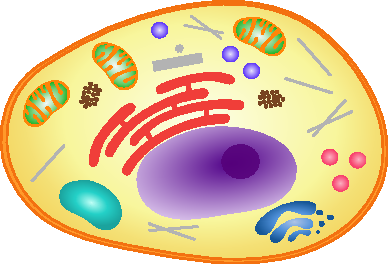
\includegraphics[width=1\linewidth]{Figures/cell.pdf} 
    \end{column}
    \begin{column}[T]{0.5\textwidth} 
       \begin{itemize}
   	 \item \scriptsize Proteins are spatially organised according to function
    	\item Significant correlation between disease classes and sub-cellular localisations
	\item Abnormal protein localisation leading to the loss of functional effects in diseases
       \end{itemize}
           \end{column}
  \end{columns}
  \bigskip
\textbf{\textcolor{Blue}{Spatial proteomics}} is the systematic
    study of protein localisations.
\end{frame}


%----------------------------------------------------------------------------------------
%	SLIDE 2 ---- Localisation Maps 
%----------------------------------------------------------------------------------------

\section{Global localisation maps}

\begin{frame}{Localisation maps from quantitative proteomics}
      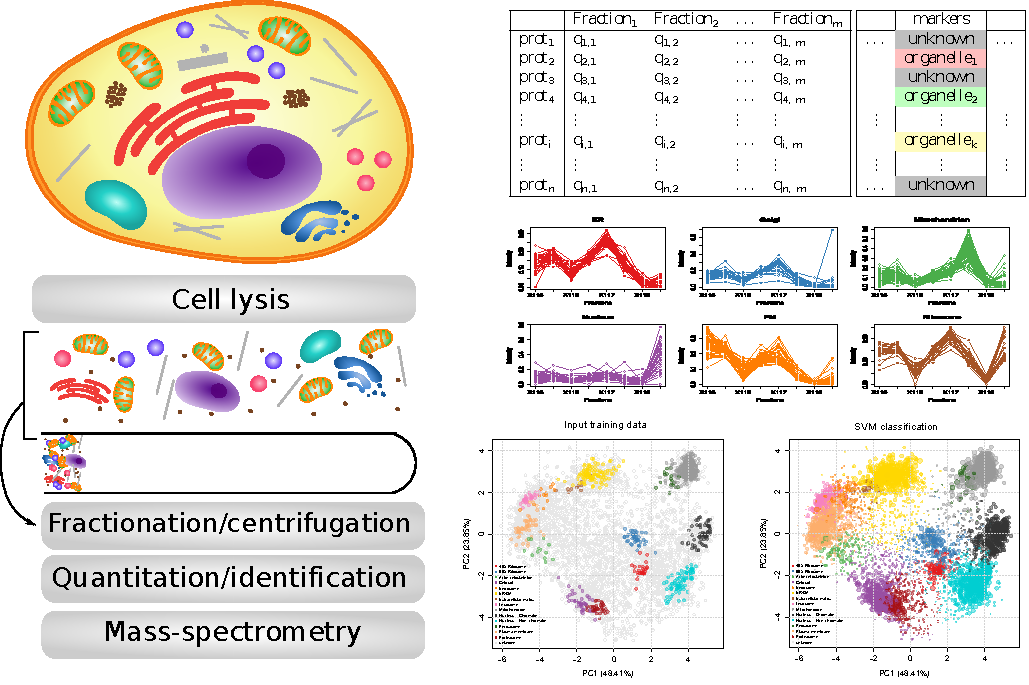
\includegraphics[width=1\linewidth]{Figures/lopit-new.pdf} 
\end{frame}
  
        

%----------------------------------------------------------------------------------------
%	SLIDE 3 ---- Other sources of information
%----------------------------------------------------------------------------------------

\begin{frame}{Sources of information}
  \vspace{0.5cm}
  \begin{centering}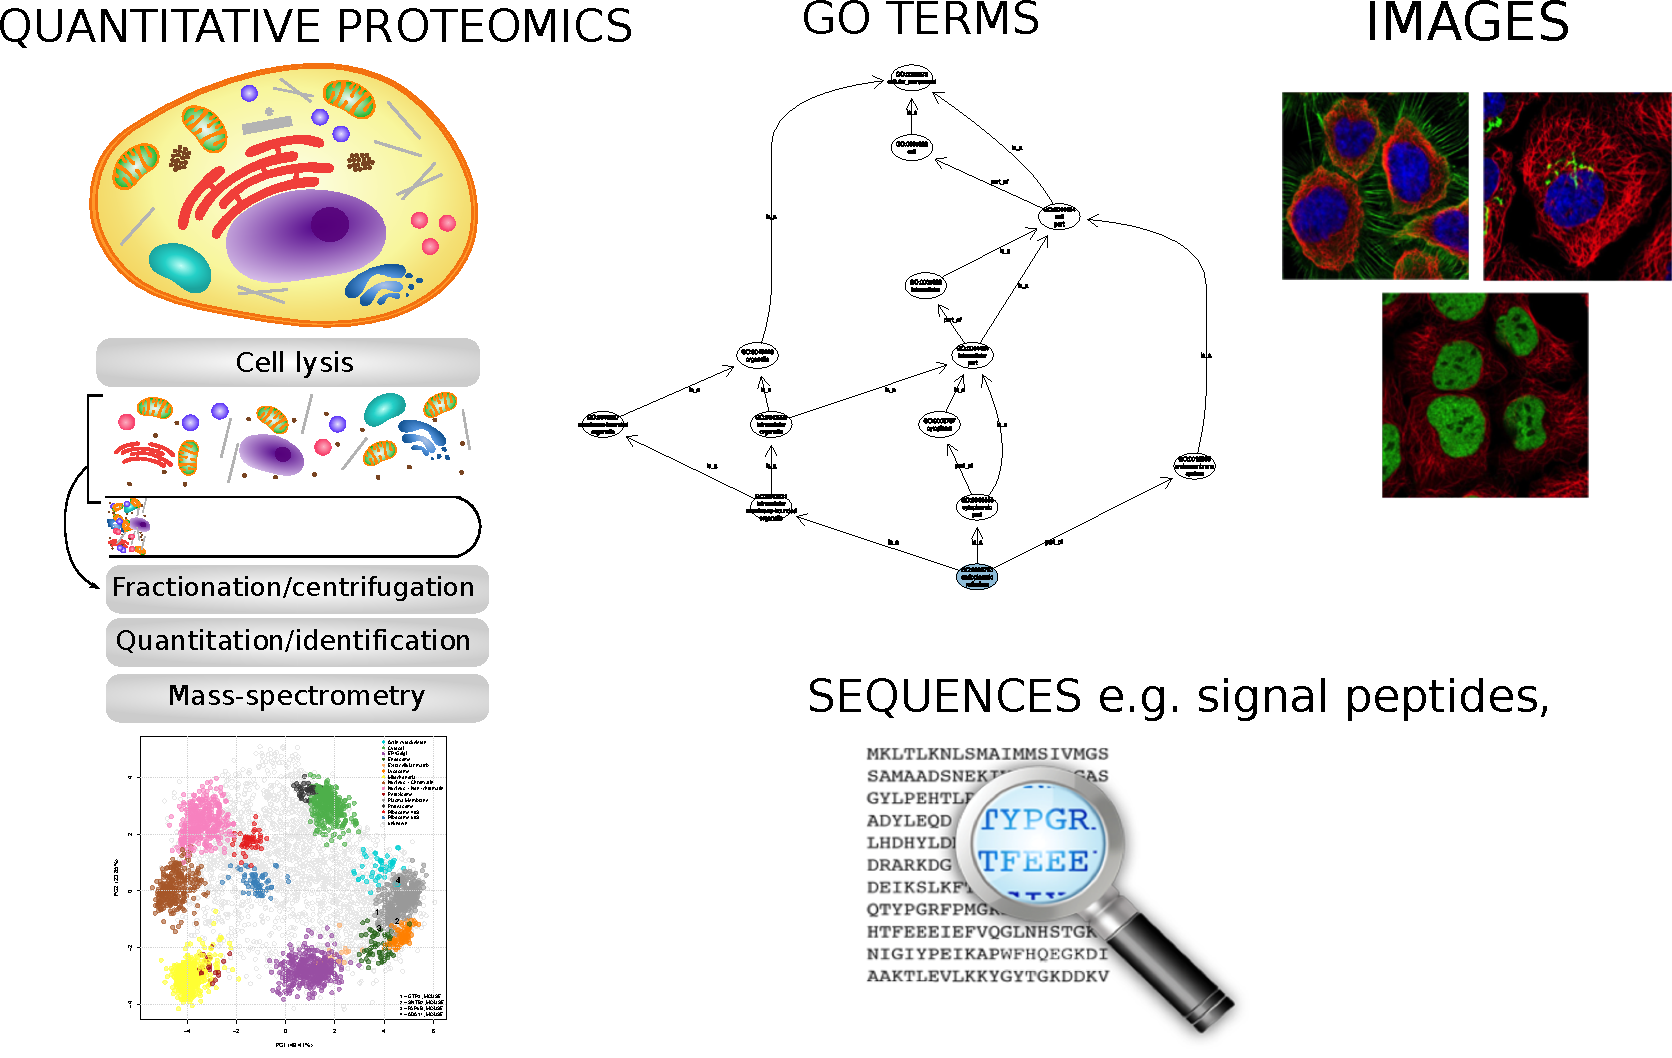
\includegraphics[width=1\linewidth]{Figures/data.pdf} 
  \end{centering} 
  \vspace{0.7cm}
\end{frame}

%----------------------------------------------------------------------------------------
%	SLIDE 4 ---- Combining data - our goal
%----------------------------------------------------------------------------------------

\begin{frame}

  \begin{block} \large \textcolor{Blue}{Goal: to pinpoint the sub-cellular localisation of proteins}
  Support/complement the primary target domain (experimental data)
  with auxiliary data (e.g. annotation) features without compromising the
  integrity of our primary data.
  \end{block}
  \bigskip
  
  \begin{block}{How - Transfer Learning}
  \begin{itemize}
  \item Drawing on data from a related/auxiliary domain to solve a primary learning task
  \end{itemize}
  \end{block}

\end{frame}

%----------------------------------------------------------------------------------------
%	SLIDE 8 ---- The classifiers
%----------------------------------------------------------------------------------------

\begin{frame}

  \begin{columns}[t]
    \begin{column}[T]{0.5\textwidth}\textcolor{Blue}{KNN TL}: class-specific weights\\
    \scriptsize{If $\hat{\bp}_u$
and $\hat{\bq}_u$, represent the distribution of classes among the sets of nearest 
neighbours for each protein for P and A, then the voting scores for each
class $i \in C$ are calculated as \begin{equation*} V(i) = \theta_i
\hat{p}_i^u + (1 - \theta_i) \hat{q}_i^u \label{vtheta} \end{equation*}
and the protein is assigned to the class $c \in C$ maximizing $V(i)$
\[ c = \operatorname*{arg\,max}_i V(i) .  \] The class weights
$\theta_i$ in equation \ref{vtheta} control the relative importance of
the two types of neighbours for each class $i \in C$.}

\vspace{2cm}

{\tiny Adapted from Wu \& Dietterich (ICML '04) - transfer learning with $k$-NNs and SVMs}

    \end{column}
    
    \begin{column}[T]{0.5\textwidth}\textcolor{Blue}{SVM TL}: data-specific kernels/parameters\\
        \scriptsize{We adjust the classical SVM machinery and introduce a
separate kernel $K^A$ and parameter vector $\bal_A$ for the auxilliary
data. An instance to be classified now contains both P and A data. The latent function becomes \[ f(\bx,
\bv; \bal_P, \bal_A, b) =  \]  \[ \sum_{l=1}^m y_l \left[ \alpha_l^P
K^P(\bx_l, \bx) + \alpha_l^A K^A(\bv_l, \bv) \right] + b \] and
training requires us to solve the linear program \begin{equation*}
\min_{\bal_P,\bal_A,\bxi,b} |\alpha_P|_1 + |\alpha_A|_1 + C|\xi|_1
\label{ob2} \end{equation*} such that for each $i = 1,\ldots,m$ \[ y_i
f(\bx_i, \bv_i; \bal_P, \bal_A, b) + \xi_i \geq 1 \] and $\bal_P,
\bal_A, \bxi \geq \bm{0}$.}
    \end{column}
    
  \end{columns}
\end{frame}

%----------------------------------------------------------------------------------------
%	SLIDE 5 ---- Transfer learning with k-NN and SVMs
%----------------------------------------------------------------------------------------

\begin{frame}{Biological application}
Localise proteins in mouse e14 pluripotent stem cells
    
  \begin{figure}
    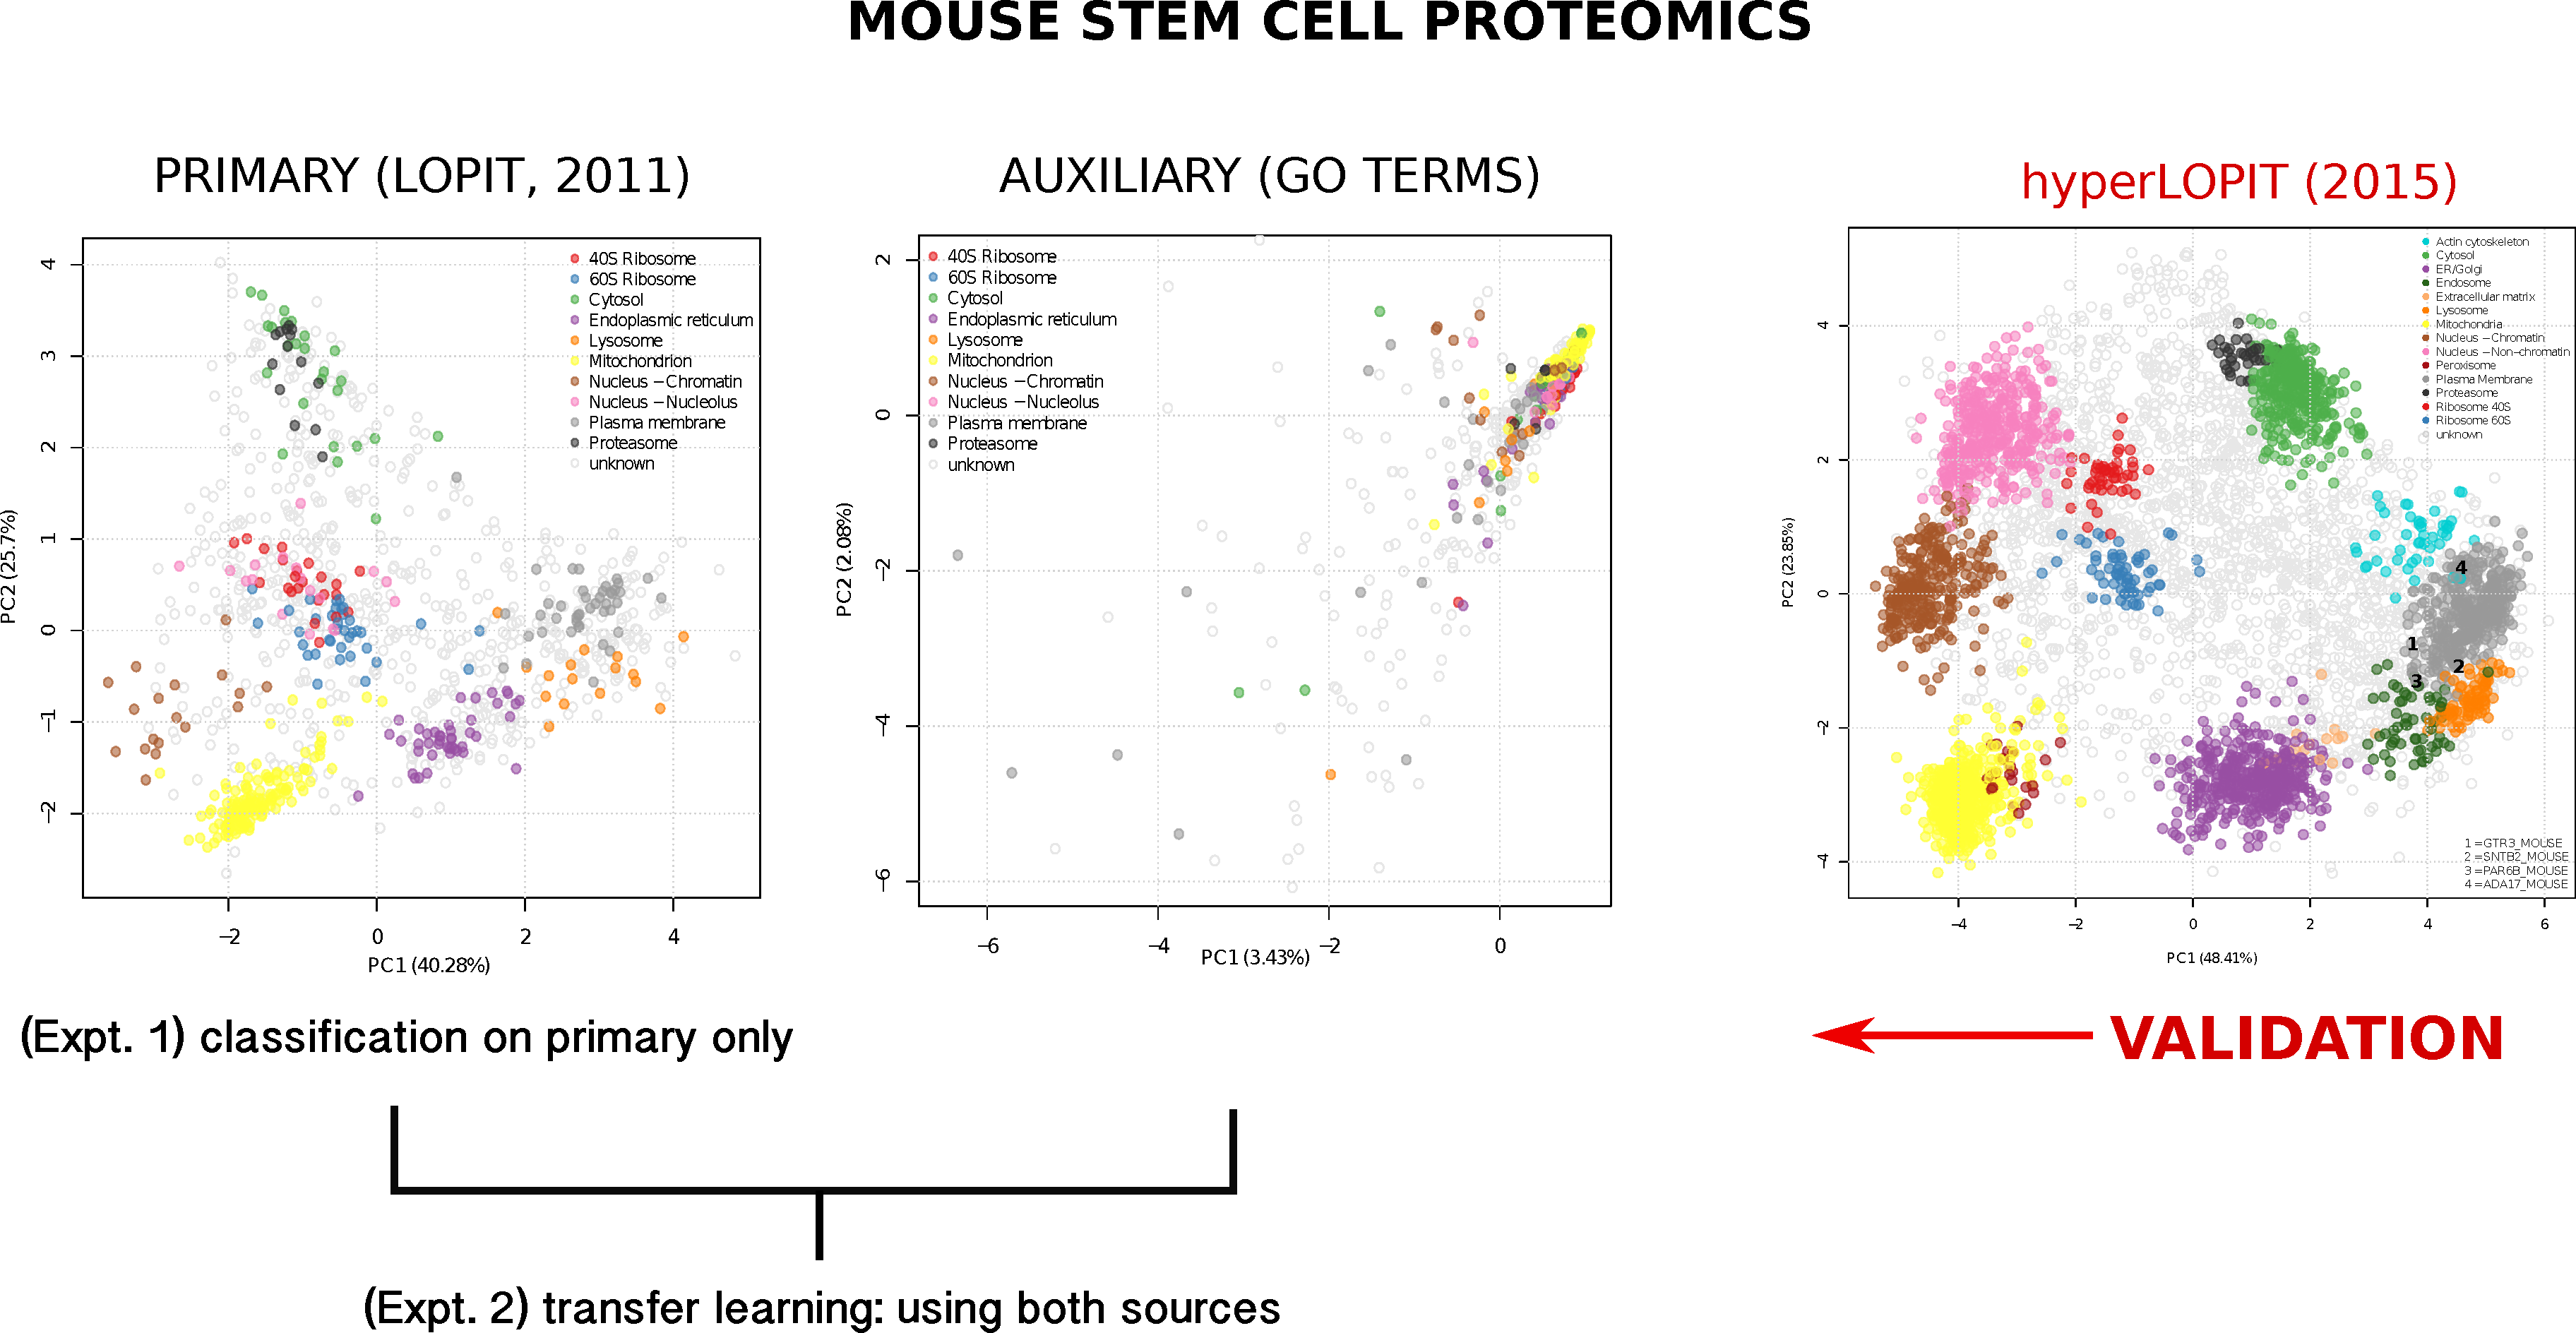
\includegraphics[width=1\linewidth]{Figures/old-new2.pdf}
  \end{figure}
\end{frame}




%----------------------------------------------------------------------------------------
%	SLIDE 7 ---- Increased discrimination power
%----------------------------------------------------------------------------------------

\begin{frame}{Results: application to mouse stem cells}
  \begin{figure}
    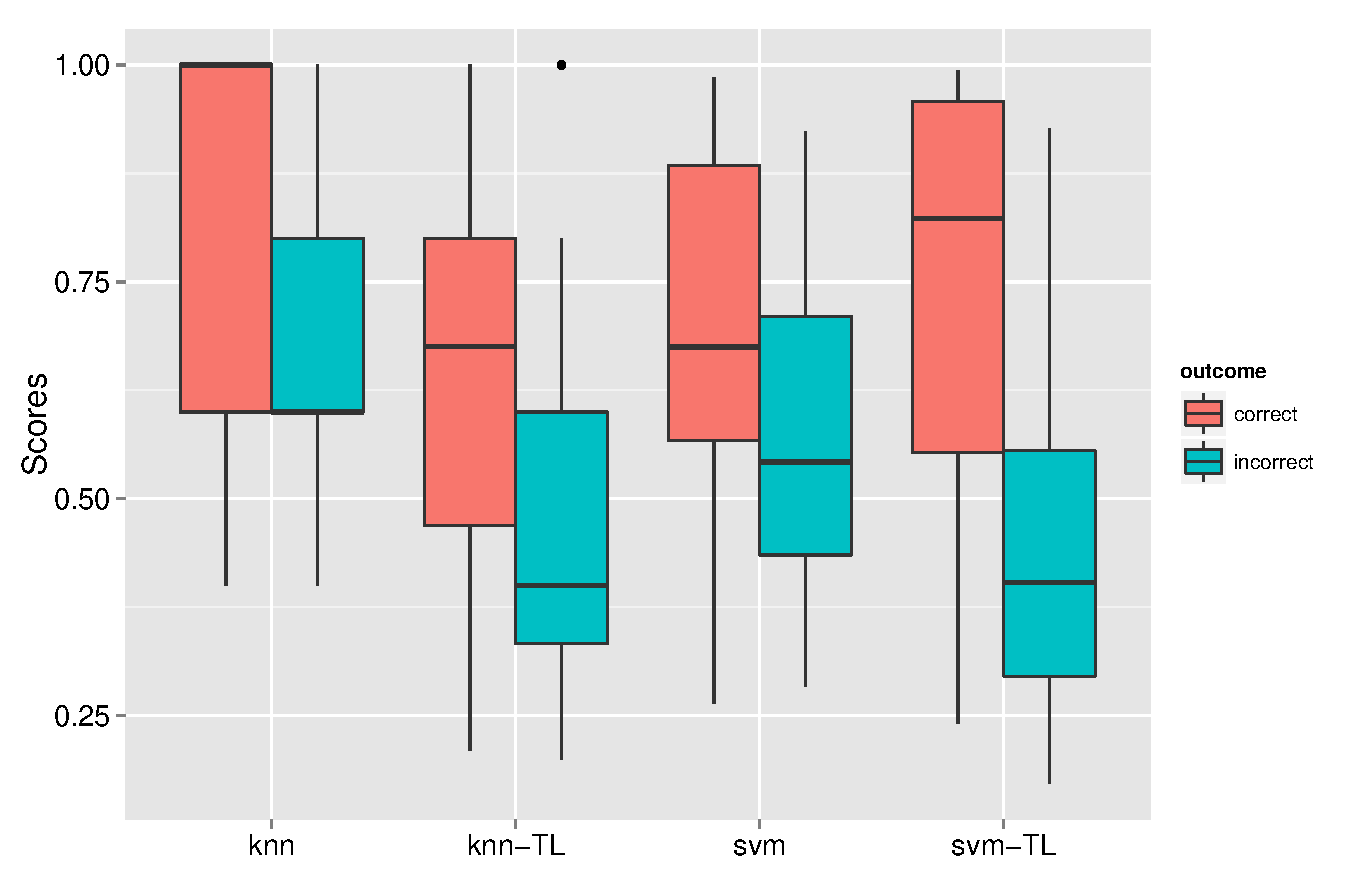
\includegraphics[width=.9\linewidth]{Figures/classifierDiscriminationPowerk5.pdf}
  \end{figure}
\end{frame}


%----------------------------------------------------------------------------------------
%	Acknowledgements
%----------------------------------------------------------------------------------------
  \begin{frame}

   \begin{block}{Software}
     \vspace{.1cm}
    Infrastructure: \Rpackage{MSnbase}, ML: \Rpackage{pRoloc} and data: \Rpackage{pRolocdata}.
    \vspace{.2cm}
  \end{block}
   
  \begin{block}{Pre-print}
  \begin{small}
    \textit{Learning from heterogeneous data sources: an application
      in spatial proteomics.} Breckels LM, Holden S, Wonjar D, Mulvey
    CM, Christoforou A, Groen AJ, Kohlbacher O, Lilley KS and Gatto L.
    bioR$\chi$iv~pre-print~\url{http://dx.doi.org/10.1101/022152}
    \vspace{.2cm}
    \end{small}
  \end{block}
  
  \begin{block}{Acknowledgements}
    \begin{itemize}
    \item Laurent Gatto, CPU, Kathryn Lilley, CCP
    \item Funding: BBSRC
    \end{itemize}
  \end{block}
  
  \footnotesize{Slides available under CC-BY license:
    \url{http://dx.doi.org/10.6084/m9.figshare.1619711}.}
  
  \end{frame}

\end{document}
